\فصل{مطالب تکمیلی}

\قسمت{شبکهٔ مسیر و آزمون‌های تکمیلی آرایش}

\label{sec:appendix-parametric-particle}

\زیرقسمت{آموزش شبکهٔ مسیر}

شکل~\ref{fig:appendix-formation-training} نتایج این بررسی را نشان می‌دهد.
مسیر آموزش برای دو مؤلفهٔ باقیمانده جداگانه رسم شده است.
پس از آموزش عرضی، وزن‌های آن بخش ثابت ماندند.
گام ثبت‌شدهٔ انتخاب وزن ۴۸۰۸ است.

\begin{figure}[htbp]
\centering
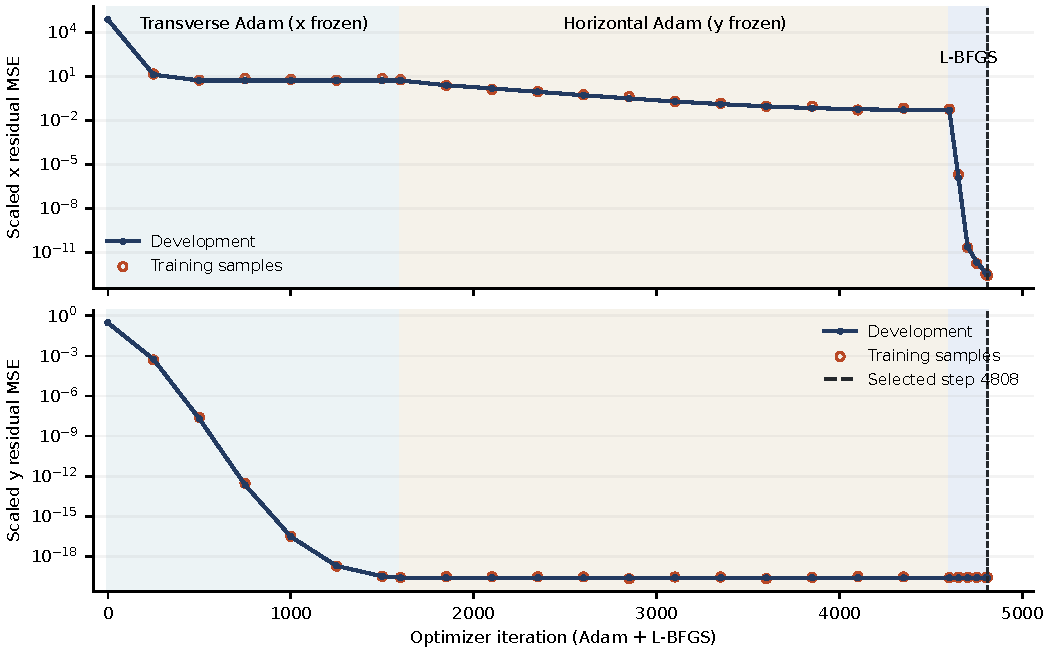
\includegraphics[width=\linewidth,height=.72\textheight,keepaspectratio]{figs/parametric_particle_pinn/P04_training.pdf}
\caption{باقیماندهٔ آموزش و توسعه در مراحل برازش شبکهٔ مسیر.}
\label{fig:appendix-formation-training}
\end{figure}

\زیرقسمت{برش شرایط رهاسازی}

شکل~\ref{fig:appendix-formation-release-slices} نتایج این بررسی را نشان می‌دهد.
برش‌های رهاسازی، ۱۰۰۷ حالت جدا از مجموعهٔ آزمون اصلی را پوشش دادند.
مکان محوری اولیه در همهٔ برش‌ها $0.66$ است.
سرعت محوری اولیه در برش داخلی $0.35$ است.
ضربدرها پایان مسیر پیش از پرس‌وجوی $t^*=1$ را نشان می‌دهند.
خطای هر خانه از بازهٔ مشترک معتبر محاسبه شده است.

\begin{figure}[htbp]
\centering
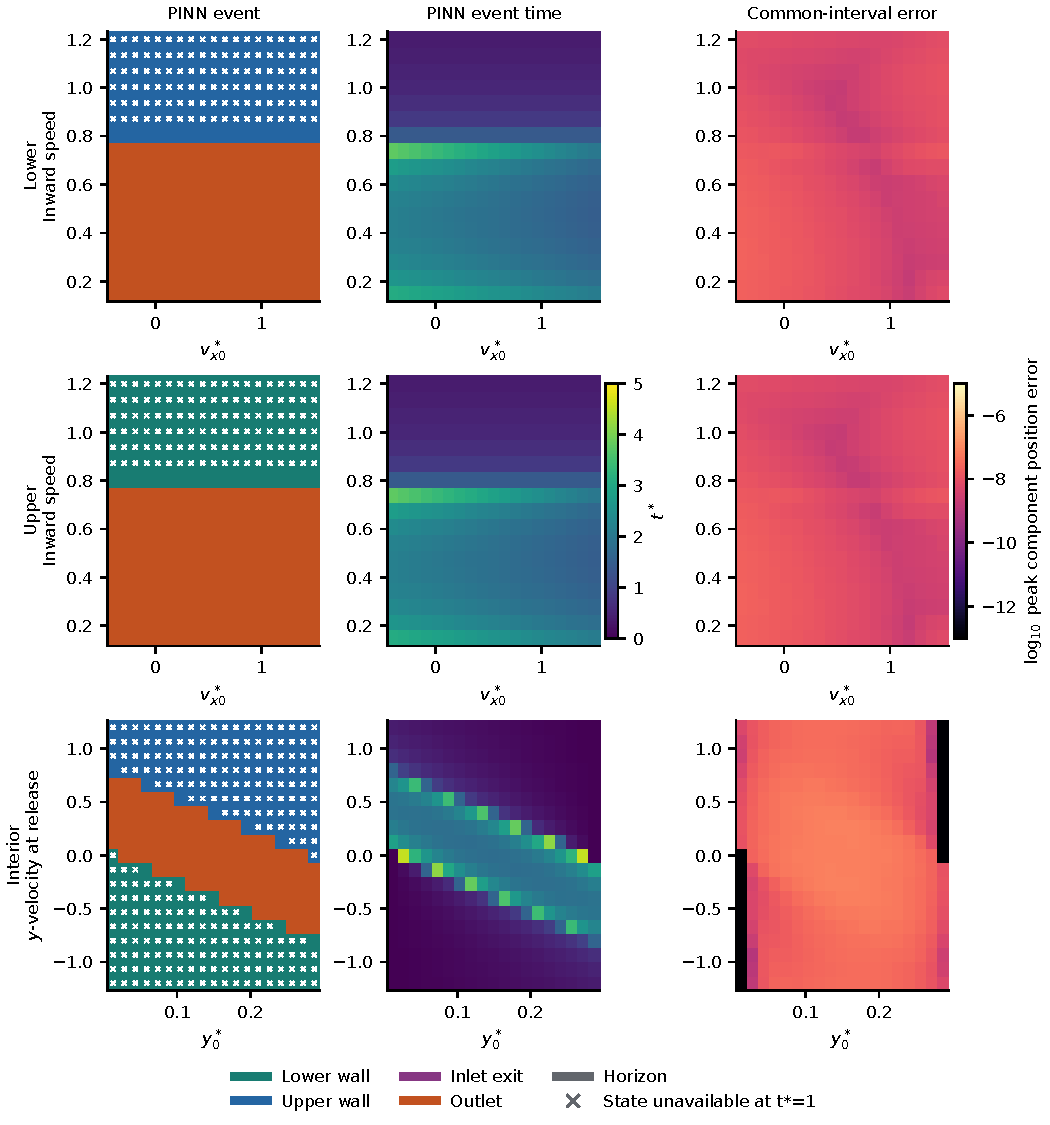
\includegraphics[width=\linewidth,height=.72\textheight,keepaspectratio]{figs/parametric_particle_pinn/P05_release_slices.pdf}
\caption[بازهٔ معتبر و خطای پیش‌بینی برای برش‌های شرایط اولیه.]{بازهٔ معتبر و خطای پیش‌بینی برای برش‌های شرایط اولیه.}
\label{fig:appendix-formation-release-slices}
\end{figure}

\زیرقسمت{هندسهٔ هدف}

شکل~\ref{fig:appendix-formation-geometry} نتایج این بررسی را نشان می‌دهد.
برای استادیوم کوچک، مکان مرکز هدف در نه حالت تغییر کرد.
\ReviewGold{از ۲۷ اجرا، ۲۴ برنامه پذیرفته شدند.}
برای بیضی، هفت ترکیب نسبت محورها و زاویه بررسی شد.
همهٔ ۲۱ اجرای بیضی در بازهٔ آزموده‌شده پذیرفته شدند.
این آزمون‌ها با شش پرتابگر ثابت انجام شدند.

\begin{figure}[htbp]
\centering
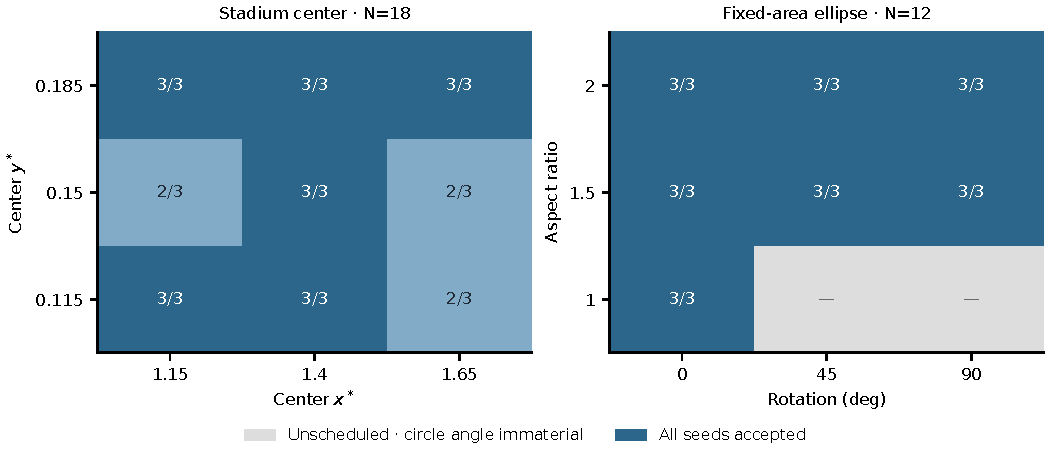
\includegraphics[width=\linewidth,height=.72\textheight,keepaspectratio]{figs/parametric_particle_pinn/F04_geometry_slices.pdf}
\caption[پذیرش آرایش برحسب مرکز هدف و شکل بیضی.]{\ReviewGold{پذیرش آرایش برحسب مرکز هدف و شکل بیضی.}}
\label{fig:appendix-formation-geometry}
\end{figure}

\زیرقسمت{نمونه‌های آرایش}

شکل~\ref{fig:appendix-formation-gallery} نتایج این بررسی را نشان می‌دهد.
هدف‌های ماهی و پیکان هرکدام ۲۴ ذره داشتند.
برای هر هدف، هر سه اجرای چیدمان شش‌پرتابگری پذیرفته شدند.
نمونهٔ استادیوم ۷۲ ذره‌ای از یک اجرای پذیرفته‌شدهٔ رهاسازی آزاد است.

\begin{figure}[htbp]
\centering
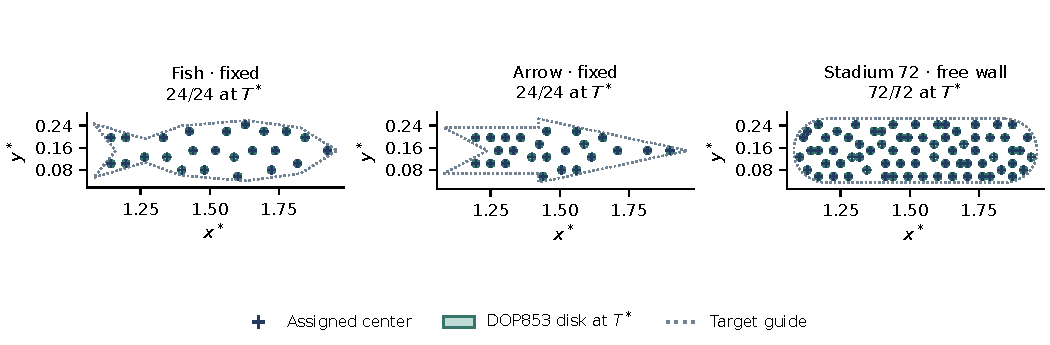
\includegraphics[width=\linewidth,height=.72\textheight,keepaspectratio]{figs/parametric_particle_pinn/F08_shape_gallery.pdf}
\caption{بازپخش هدف ماهی، پیکان و استادیوم در زمان هدف.}
\label{fig:appendix-formation-gallery}
\end{figure}

\زیرقسمت{چیدمان قرینه}

شکل~\ref{fig:appendix-formation-reflection} نتایج این بررسی را نشان می‌دهد.
دو چیدمان پرتابگر برای یک هدف ۱۸ ذره‌ای مقایسه شدند.
\ReviewGold{چیدمان اصلی و قرینه به‌ترتیب دو و سه اجرای پذیرفته‌شده داشتند.}
این شمارها عملکرد دو چیدمان را در سه اجرای ثبت‌شده توصیف می‌کنند.

\begin{figure}[htbp]
\centering
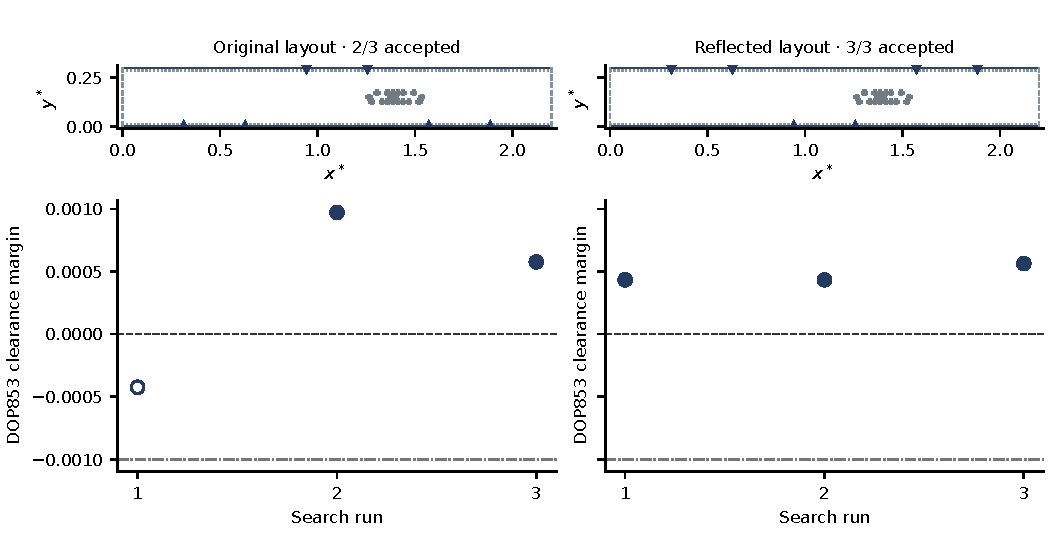
\includegraphics[width=\linewidth,height=.72\textheight,keepaspectratio]{figs/parametric_particle_pinn/F09_reflection.pdf}
\caption[مقایسهٔ دو چیدمان قرینه با هدف مشترک ۱۸ ذره‌ای.]{\ReviewGold{مقایسهٔ دو چیدمان قرینه با هدف مشترک ۱۸ ذره‌ای.}}
\label{fig:appendix-formation-reflection}
\end{figure}
